\documentclass[border=10pt]{standalone}
\usepackage{tikz}
\usetikzlibrary{shapes,backgrounds,calc,patterns,trees}

\begin{document}
	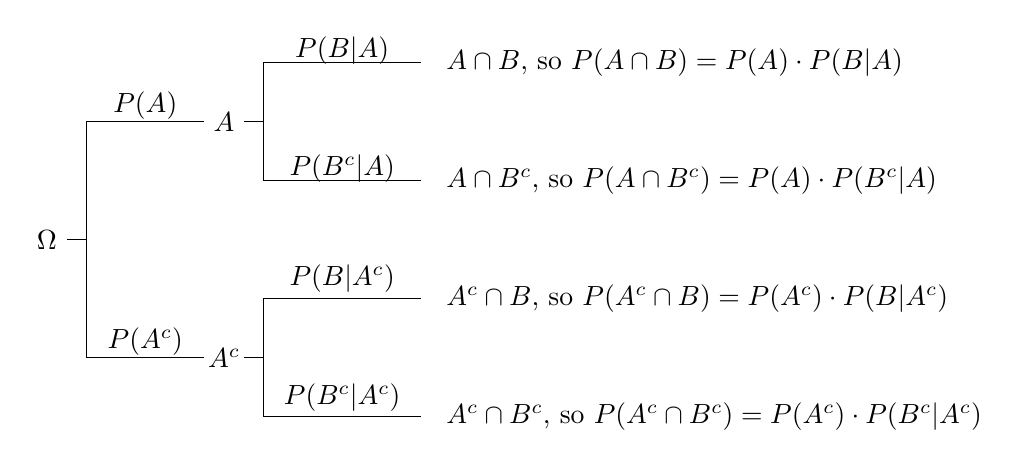
\begin{tikzpicture}
		\node at (.25,0) {\(\Omega\)};
		\draw (.5,0) -- (.75,0);
		\draw (.75,1.5) -- (.75,-1.5);
		\draw (.75,1.5) -- (2.25,1.5);
		\node at (1.5,1.7) {\(P(A)\)} ;
		\node at (2.5, 1.5) {\(A\)};
		\draw (.75,-1.5) -- (2.25,-1.5);
		\node at (1.5,-1.3) {\(P(A^c)\)} ;
		\node at (2.5, -1.5) {\(A^c\)};
		
		\draw (2.75,1.5) -- (3,1.5);
		\draw (2.75,-1.5) -- (3,-1.5);
		
		\draw (5,.75) -- (3,.75) -- (3,2.25) -- (5,2.25);
		\draw (5,-.75) -- (3,-.75) -- (3,-2.25) -- (5,-2.25);
		
		\node at (4,2.4) {\(P(B\vert A)\)};
		\node at (4,.9) {\(P(B^c\vert A)\)};
	
		\node at (4,-2) {\(P(B^c\vert A^c)\)};
		\node at (4,-.5) {\(P(B\vert A^c)\)};	
		
		\node[right] at (5.2, 2.25) {\(A\cap B\), so \(P(A\cap B)=P(A) \cdot P(B\vert A)\)};
		\node[right] at (5.2, .75) {\(A\cap B^c\), so \(P(A\cap B^c) = P(A) \cdot P(B^c\vert A)\)};
		\node[right] at (5.2, -.75) {\(A^c \cap B\), so \(P(A^c\cap B) = P(A^c)\cdot P(B\vert A^c) \)};
		\node[right] at (5.2, -2.25) {\(A^c \cap B^c\), so \(P(A^c \cap B^c) = P(A^c)\cdot P(B^c\vert A^c)\)};
	
	\end{tikzpicture}
\end{document}

